\documentclass[12pt, a4paper]{report}
% !TEX root = holder_file.tex
\makeatletter\@addtoreset{chapter}{part}\makeatother%
\usepackage[dvipsnames]{xcolor}
\usepackage{verbatim}
\usepackage{graphicx}
\usepackage{geometry}
\definecolor{myblue}{rgb}{0.058, 0.588, 0.558}
\definecolor{whpaste}{rgb}{0.180,0.211,0.178}
\definecolor{Pastel Blue}{HTML}{AADDEE}
\definecolor{foo}{HTML}{EFF5F9}

\usepackage{tcolorbox}
%%------------------------
\usepackage{nicematrix}
\usepackage{url} % typeset URL's reasonably
\usepackage{listings}
\usepackage{fancybox}
\usepackage{subfigure}
\usepackage{epsfig}
\usepackage{color}
\usepackage{eurosym}
\usepackage{amsmath,amssymb,amsthm,mathrsfs,amsfonts}
\usepackage{wasysym}
%\usepackage{MnSymbol}
\usepackage{amssymb,latexsym, bbm,comment}
\usepackage{colortbl}
\usepackage{fancyhdr}
\usepackage{tikz}
\usepackage{bbm,dsfont}
\newcommand{\amount}{6in}   %%<---- adjust
\usepackage{float}
\usepackage{esvect}
\usepackage{mathtools}
\usepackage{calligra}
\usepackage[T1]{fontenc}
\usepackage[onehalfspacing]{setspace}
\usepackage{booktabs}
\usepackage{array} 
%\usepackage{cancel, caption, mathtools, subcaption, amsthm}
\usepackage{caption}
\usepackage{float}
\usepackage{refstyle}

%----------- something for maths ----------
\geometry{
	left=1.42in,
	right=1.1in,
	top=1.4in,
	bottom=1.4in
}
%%------------------------
%%defination add korar jonno egula likhsi
{\theoremstyle{plain}
	\newtheorem{definition}{Definition}[section]
	\newtheorem{lemma}[definition]{Lemma}
	\newtheorem{theorem}[definition]{Theorem}
	\newtheorem{cor}[definition]{Corollary}
	\newtheorem{proposition}[definition]{Proposition}
	\newtheorem*{condition}{Condition}
}{\theoremstyle{definition}
	\newtheorem{example}[definition]{Example}
	\newtheorem{exercise}[definition]{Exercise}
	\newtheorem{remark}[definition]{Remark}
	\newcommand\dlim{\displaystyle \lim}
	\newcommand\dsum{\displaystyle \sum}
	\newcommand\dint{\displaystyle \int}
	\newcommand\N{\mathbb{N}}
	\newcommand\R{\mathbb{R}}
	\newcommand\Z{\mathbb{Z}}
	\newcommand\F{\mathcal{F}}
	\newcommand\E{\mathbb{E}}
	\newcommand\V{\mathbb{V}}
	\newcommand\pr{\mathbb{P}}
	\newcommand\Q{\mathbb{Q}}
	%\newcommand\lub{\text{lub}}
	\newcommand\dss{\displaystyle}
	\newcommand\pbs{(\Omega, \mathscr{F}, \pr)}
	\newcommand\mycol{\textcolor{red!70!black!40}}
	\newcommand\bst{$\circleddash$}
	%\newcommand\dfncol{\textcolor{green}}
	\newcommand\exmcol{\textcolor{red}}
	\newcommand\thmcol{\textcolor{blue}}
	\newcommand\dfnline{\rule{0.99\linewidth}{1.2pt}}
	%%%%%%% chapter color 
	\newcommand{\sub}{\textcolor{black}}
	\newcommand{\sect}{\textcolor{black}}
	%\newcommand{\sect}{\textcolor{green!148!blue!137}}
	\newcommand{\chap}{\textcolor{black}}
	%%%%%%%%%%%%%%%
	\definecolor{rahmen}{RGB}{0,73,114}
	\definecolor{grund}{RGB}{238,241,251}          
	\definecolor{schrift}{RGB}{0,73,114}
	
	%%%%%  for code
	\usepackage{listings}
	\usepackage{xcolor}
	%%%%% for code design %%%%%%%%
	\definecolor{codegreen}{rgb}{0,0.6,0}
	\definecolor{codegray}{rgb}{0.5,0.5,0.5}
	\definecolor{codepurple}{rgb}{0.58,0,0.82}
	\definecolor{backcolour}{rgb}{0.95,0.95,0.92}
	
	\lstdefinestyle{mystyle}{
		backgroundcolor=\color{backcolour},  
		commentstyle=\color{codegreen},
		keywordstyle=\color{magenta},
		numberstyle=\tiny\color{codegray},
		stringstyle=\color{codepurple},
		basicstyle=\ttfamily\footnotesize,
		breakatwhitespace=false,        
		breaklines=true,                
		captionpos=b,                    
		keepspaces=true,                
		numbers=left,                    
		numbersep=5pt,                  
		showspaces=false,                
		showstringspaces=false,
		showtabs=false,                  
		tabsize=2
	}
	
	\lstset{style=mystyle}
	%%%%%%
	
	\newcommand{\ito}{It$\hat{\text{o}}$ }
	
\begin{document}
	% !TEX root = holder_file.tex

%\vspace{5cm}
\thispagestyle{empty}
\begin{center}
	%\rule{\textwidth}{1.6pt}\vspace*{2pt} 
	\textcolor{blue!60!black!80}{\Large\bf A COMPREHENSIVE STUDY OF OPTIONS PRICING BY}
	\textcolor{blue!60!black!80}{{\Large\bf MONTE CARLO METHODS\\}}
	%\rule{\textwidth}{1.6pt}\vspace{-\baselineskip}\vspace{2pt}
	\rule{\textwidth}{0.4pt}
	\textcolor{blue!60!black!100}{\it A project submitted to University of Dhaka in partial fulfillment of the requirements for the degree of Science of Applied Mathematics}
	\vspace{.4in}
\end{center}
\begin{center}
	\textcolor{blue!60!black!80}{\bf FORTH YEAR(HONS.)PROJECT 2020}\\
	\vspace{3pt}
	{COURSE NO.: AMTH-460}
\end{center}
\vspace{.3in}
\begin{center}
		\textcolor{blue!60!black!80}{\it Submitted By:}\\[2mm]
	\begin{tabular}{ c c c}
		{\bf Class Roll} & :& \hspace{0.3in}SN-020-035  \\ 
		{\bf Registration No.} &: & \hspace{0.4in}2017-414-047  \\  
		{\bf Session} & :&2017-18     
	\end{tabular}
	
	\vspace{.6in}
\end{center}

\begin{figure}[H]
	\centering
	
\includegraphics[width=.25\linewidth]{logo}
\end{figure}

%\begin{figure}[!htb]
%	\begin{center}
%		
\includegraphics[width=0.8\textwidth]{logo}
%	\end{center}
%\end{figure}

\begin{center}
	{\bf Department of Applied Mathematics\\
	University of Dhaka}\\
    \today
\end{center}
	% !TEX root = holder_file.tex

%\vspace{5cm}
\thispagestyle{empty}
\begin{center}
	%\rule{\textwidth}{1.6pt}\vspace*{2pt} 
	\textcolor{blue!60!black!80}{\Large\bf A COMPREHENSIVE STUDY OF OPTIONS PRICING BY}
	\textcolor{blue!60!black!80}{{\Large\bf MONTE CARLO METHODS\\}}
	%\rule{\textwidth}{1.6pt}\vspace{-\baselineskip}\vspace{2pt}
	\rule{\textwidth}{0.4pt}
	\textcolor{blue!60!black!100}{\it A project submitted to University of Dhaka in partial fulfillment of the requirements for the degree of Science of Applied Mathematics}
	\vspace{.4in}
\end{center}
\begin{center}
	\textcolor{blue!60!black!80}{\bf FORTH YEAR(HONS.)PROJECT 2020}\\
	\vspace{3pt}
	{COURSE NO.: AMTH-460}
\end{center}
\begin{center}
	\textcolor{blue!60!black!80}{\bf SUPERVISED BY}\\
	\vspace{3pt}
	{Dr. A B M Shahadat Hossain}\\
		{Associate Professor,
			Department of Applied Mathematics}
\end{center}
\vspace{.3in}
\begin{center}
	\textcolor{blue!60!black!80}{\it Submitted By:}\\[2mm]
	KRISHNA BANIK PUSHPITA\\[2mm]
	\begin{tabular}{ c c c}
		{\bf Class Roll} & :& \hspace{0.3in}SN-020-035  \\ 
		{\bf Registration No.} &: & \hspace{0.4in}2017-414-047  \\  
		{\bf Session} & :&2017-18     
	\end{tabular}
	
	\vspace{.6in}
\end{center}

\begin{figure}[H]
	\centering
	
\includegraphics[width=.25\linewidth]{logo}
\end{figure}

%\begin{figure}[!htb]
%	\begin{center}
	%		
\includegraphics[width=0.8\textwidth]{logo}
	%	\end{center}
%\end{figure}

\begin{center}
	{\bf Department of Applied Mathematics\\
		University of Dhaka}\\
\end{center}
	% !TEX root = holder_flie.tex
%\thispagestyle{empty}
\begin{abstract}
	Our main objective in this project is to introduce the Monte Carlo algorithm in the context of option pricing. Because the simulation technique is used in various domains particularly in Financial Mathematics. Here we evaluate stock price, option price using tons of versions of MC method. Now, we have described this method for European, American and Barrier options respectively and showed some efficient method for reducing its computation time and increasing accuracy. For numerical results and graphical interpretation, we have used Python Language and shown their comparison with Black-Scholes Method. 
\end{abstract}
	\tableofcontents
	\listoffigures
	\listoftables
	% !TEX root = holder_file.tex
\newpage
\noindent{\bf \Large Notations}\\[3ex]
\begin{center}
	\begin{tabular}{l*{1}{c}l}
		$a\vee b$ & : &  $\max\{a, b\}$ (i.e. the maximum of $a$ and $b$ )\\[1ex]
		
		a.e. & : & almost everywhere\\[1ex]
		a.s.           & : & almost surely, or $P-a.s$ surely , or with probability 1 \\[1ex]
		ms           & : & mean square\\[1ex]
		$\sigma(\mathcal{C})$     & : & the $\sigma$-algebra generated by $\mathcal{C}$ \\[1ex]
		$\pbs$ & : & Probability space.\\[1ex]
		$\Omega$ &:& Sample Space\\[1ex]
		$X$ &:& Random variable\\[1ex]
		$X_t$ &:& Stochastic Process\\[1ex]
		$\dss\text{as}-\lim_{n\to\infty} X_t$ &:& The almost sure limit of $X_t$\\[1ex]
	\end{tabular}
\end{center}

	% !TEX root = holder_file.tex
\chapter{Introduction}
\noindent In today's world, derivatives are frequently used in the financial markets. A financial instrument known as a derivative is one whose value is based on the cost of an underlying variable. Risk hedging, speculation, and arbitrage are all possible uses of derivatives. Futures contracts, forward contracts, options, and swaps are a few examples of common derivatives. Here, we'll talk about possibilities, including American and European ones and will suggest efficient methods for each in this project. \\[2mm]
\noindent A key development in contemporary finance is \textbf {Option Pricing}. In the case of option pricing, a tons of factors work behind this mechanism such as stock price, strike price, market volatility, interest rates etc. Here, the gap between the underlying security's current stock price and strike price defines the payoff. Moreover, the Market
volatility plays a vital role on option prices because it displays the potential risk
of sudden price changes within the market and the rate of interest is the return
on risk-free investments.\\[-3mm]

\noindent Black and Scholes established a European option valuation model. (1973). The development of the Black-Scholes model made substantial use of Taylor's expansion. A contract known as a European option lets the The option holder may later exercise the right to purchase or sell stocks. Unlike European options, a subset of the more common American options, permit the Anytime up until the expiration date, the holder may exercise the options. \\[2mm]
Either the option is European or American, Solving a practical problem is always a difficult task. Because practical problem means there are tons of uncertainties. So, then Numerical approaches are necessary for pricing choices in situations when analytical solutions are either not available or difficult to calculate. \\[2mm]
The objective of using Monte Carlo Method in the project is to address the pricing issue for American and European alternatives. Monte Carlo method is a computational simulations that rely on repeated random sampling to obtain numerical results. In this project, we have used risk neutral methodology in MC simulation. Using this method we evaluated the price for European Call, American Call and Barrier Put option. Then we have showed some variance reduction method for reducing the computation time and increasing the accuracy of these prices. We basically discussed in details about antithetic method for variance reduction. Afterwards, some comparison are shown with respect to Black Scholes Merton Model (BSM) in the final chapter. 
Our project is disscussed as follows:

\begin{itemize}
	\item In Chapter 2, we have disscussed about some preliminary concepts such as
	derivatives, different types of markets, contracts, traders, different types of
	options, payoffs, some basic definitions, stochastic process, Black-Scholes Model and etc.
	\item In Chapter 3, we have discussed about the history of Monte Carlo Method, concept, formula and algorithm. Then the discussion took a turn towards option pricing using MC method, variance reduction process for European Call option. Moreover, in this project some analysis has been shown on American Call option and Barrier Put option.
	\item In Chapter 4, this chapter is created focusing on only the comparison of each options.
	\item In Chapter 5, we make conclusion by comparing the outcomes from different
	methods discussed in this project.
\end{itemize}
    % !TEX root = holder_file.tex
\chapter{Preliminaries}

\label{ch: basics}
%----------  section ------------
\section{What Is a Derivative}



\begin{tcolorbox}
	%[colback={red!150!brown!20},coltitle={purple}]
	[colback=Pastel Blue]
	\begin{definition}
	A derivative is a type of financial contract whose value is determined by the value of an underlying asset, group of assets, or benchmark.
	\end{definition}
\end{tcolorbox}

 \noindent A derivative is a contract between two or more parties that can be traded on an over-the-counter (OTC) or exchange . These contracts can be utilized to transact variety of assets and come with their own set of risks. Derivatives prices are determined by fluctuations in the underlying asset. These financial securities are commonly used to gain access to specific markets and may be traded to hedge against risk. \\
 Derivatives can be employed for a position  hedging or speculate upon that direction of an underlying asset, or provide leverage to holdings. These assets are most often traded on over-the-counter (OTC) or exchanges and bought via brokerages. 

\section{Exchange-Traded Market}

\begin{tcolorbox}
	%[colback={red!150!brown!20},coltitle={purple}]
	[colback=Pastel Blue]
	\begin{definition}
		A derivatives exchange is a market in which people buy and sell formalized contracts that the exchange has defined.
	\end{definition}
\end{tcolorbox}

 \noindent Because of the advantages of having over over-the-counter (OTC) derivatives, exchange-traded derivatives have gained popularity. Standardization, liquidity, and the elimination of default risk are among the advantages.\\
 
 Futures and options have been two of the most widely traded ETFs. ETFs can be utilized to hedge exposure and speculate on a broad range of financial securities, including goods, stocks, currencies, and even rate of interest.
\section{Over-The-Counter Markets}

\begin{tcolorbox}
	%[colback={red!150!brown!20},coltitle={purple}]
	[colback=Pastel Blue]
	\begin{definition}
		 It is a network of dealers connected by phone and computer.
	\end{definition}
\end{tcolorbox}

\noindent Derivatives are not always traded on exchanges. In terms of total trading volume, the over-the-counter market has overtaken the exchange-traded market as a significant substitute for exchanges. It is a dealer network that is connected via phone and computer. Typically, trades are conducted over the phone between two financial institutions or between an institution and one of its clients (typically a corporate treasurer or fund manager). For the instruments that are traded more often, financial institutions frequently serve as market makers. As a result, they are constantly ready to provide both an offer price and a bid price (a price at which they are willing to purchase) (a price at which they are prepared to sell).
\section{Forward Contracts}
\noindent A forward contract is a rather straightforward derivative. 
\begin{tcolorbox}
	%[colback={red!150!brown!20},coltitle={purple}]
	[colback=Pastel Blue]
	\begin{definition}
		It is an agreement to purchase or sell a particular item at a specific price in the future.
	\end{definition}
\end{tcolorbox}
 \noindent A spot contract, which is a commitment to buy or sell an asset today, can be contrasted with it. In the over-the-counter market, forward contracts are traded, typically between two financial institutions or between a financial institution and one of its clients.
\section{Future Contracts}
\noindent A futures contract, like a forward contract, is an agreement between two parties to buy or sell an item at a certain price and time in the future. Futures contracts, in contrast to forward contracts, are often traded on an exchange. The exchange provides a few standardized aspects of the contract in order to facilitate trade. The exchange also offers a system that gives the two parties a guarantee that the contract will be upheld because the two parties to the contract are not necessarily acquainted.
\section{Types of Traders}
\noindent Markets for derivatives have achieved extraordinary success. The key reason is that they have a large amount of liquidity and have drawn many different kinds of traders.
Finding someone who is willing to take the other side of a contract is typically not an issue when an investor wants to take one side.
Hedgers, speculators, and arbitrageurs are the three main types of traders. Hedgers can lower their risk from probable future changes in a market variable by using derivatives. They are used by speculators to wager on the potential course of a market variable. To guarantee a profit, arbitrageurs take offsetting bets in two or more securities.
\subsection{Hedgers}

\begin{tcolorbox}
	%[colback={red!150!brown!20},coltitle={purple}]
	[colback=Pastel Blue]
	\begin{definition}
		A hedge is an expenditure  with the goal of lowering the risk of unfavorable changes in an asset's price. A hedge often entails taking an opposite or offsetting stake in a connected security.
	\end{definition}
\end{tcolorbox}


\subsection{Speculators}

\begin{tcolorbox}
	%[colback={red!150!brown!20},coltitle={purple}]
	[colback=Pastel Blue]
	\begin{definition}
		A speculator tries to outperform conventional longer-term investors by using tactics and often a shorter time horizon.
	\end{definition}
\end{tcolorbox}

\noindent Speculators assume risk in the hopes of earning profits that are significant enough to outweigh the risk, particularly when predicting future price changes.
\subsection{Arbitrageurs}

\begin{tcolorbox}
	%[colback={red!150!brown!20},coltitle={purple}]
	[colback=Pastel Blue]
	\begin{definition}
		An investor who makes an effort to capitalize on market inefficiencies is known as an arbitrageur.
	\end{definition}
\end{tcolorbox}

\noindent Prices, dividends, regulations, or any other component of the markets may be affected by these inefficiencies. Arbitrage in terms of pricing occurs most frequently.
\section{Options}
\noindent Both on exchanges and in the over-the-counter market, options are exchanged. Two different options are available.
\subsection{Call Options}

\begin{tcolorbox}
	%[colback={red!150!brown!20},coltitle={purple}]
	[colback=Pastel Blue]
	\begin{definition}
		Financial contracts known as call options grant the option buyer the right, but not the commitment, to purchase a stock, bond, commodity, or other asset or instrument at a particular price within a predetermined time window. 
	\end{definition}
\end{tcolorbox}

\noindent The underlying asset is a stock, bond, or product. When the value of the underlying asset rises, the call buyer makes money.
\subsection{Put Options}

\begin{tcolorbox}
	%[colback={red!150!brown!20},coltitle={purple}]
	[colback=Pastel Blue]
	\begin{definition}
		The contract known as a put option (or "put") grants the option purchaser the power, but not the duty, to sell—or sell short—a set amount of the underlying asset at a specified price within a given time span.
	\end{definition}
\end{tcolorbox}

\noindent The striking price is the predetermined price at which the buyer of the put option may sell the underlying security.
\subsection{Option Payoff diagram}

\begin{figure}[!htb]
	\begin{minipage}[l]{0.5\linewidth}
		\begin{center}
			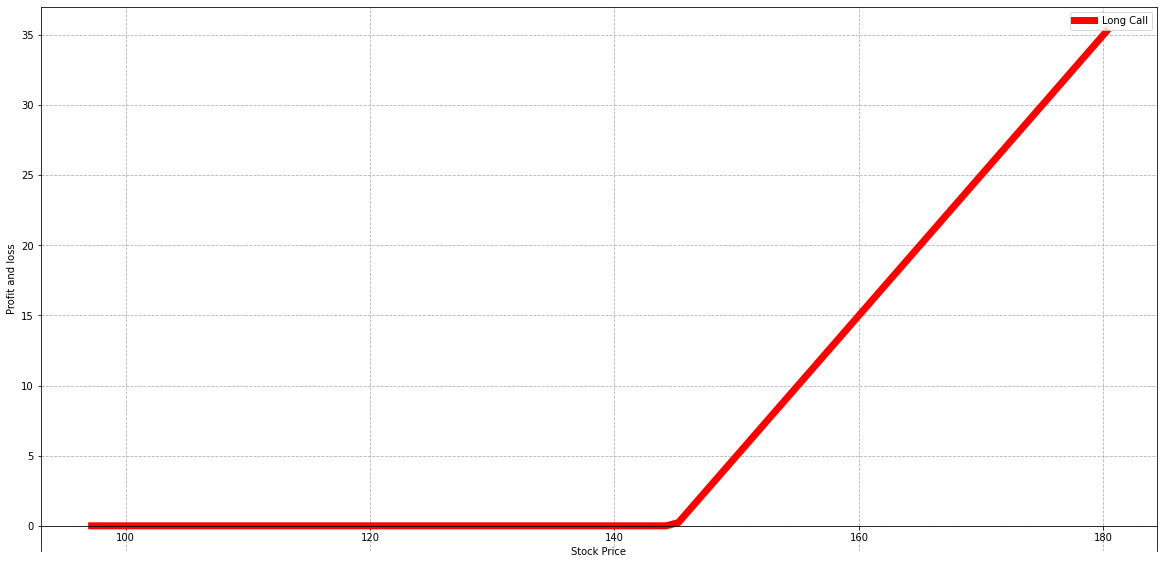
\includegraphics[width=1\textwidth]{Long_call}
		\end{center}
	\end{minipage}
	\hfill
	\begin{minipage}[r]{0.5\linewidth}
		\begin{center}
			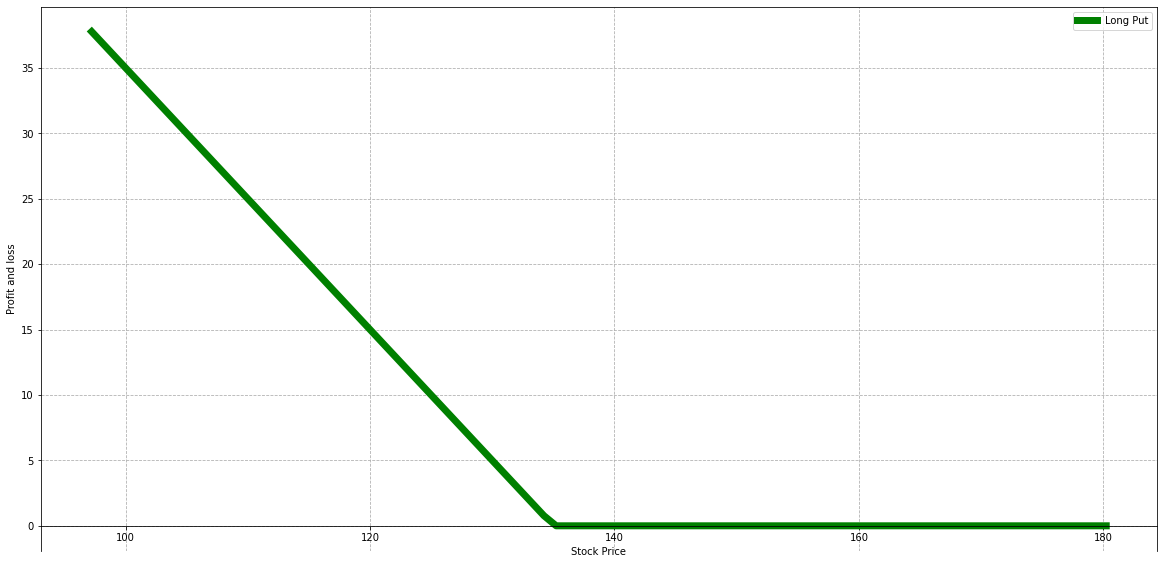
\includegraphics[width=1\textwidth]{Long_put}
		\end{center}
	\end{minipage}
	\caption{ Long Position}
\end{figure}

\begin{figure}[!htb]
	\begin{minipage}[l]{0.5\linewidth}
		\begin{center}
			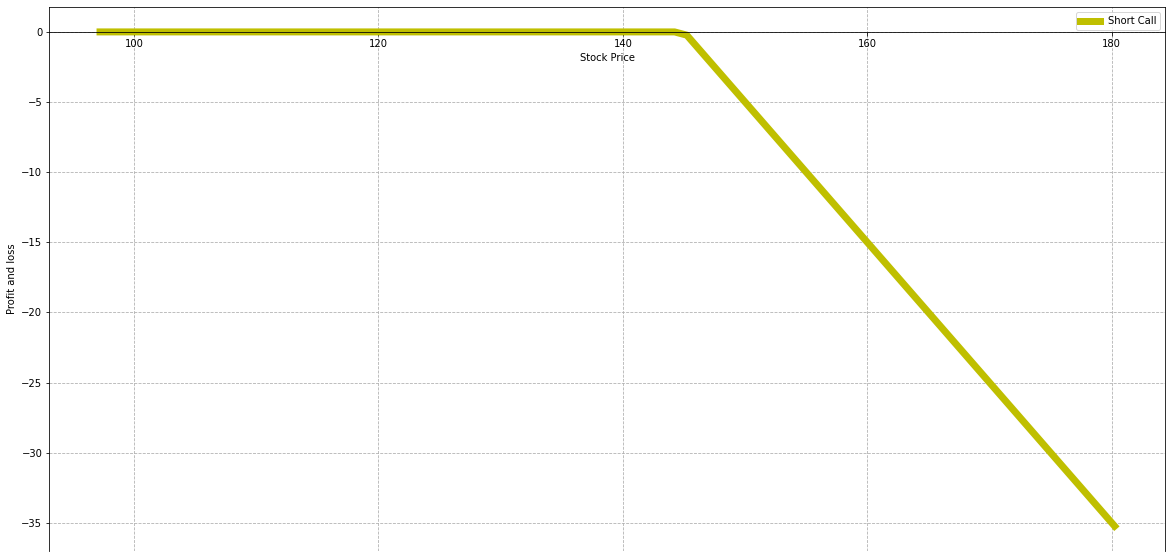
\includegraphics[width=1\textwidth]{Short_call}
		\end{center}
	\end{minipage}
	\hfill
	\begin{minipage}[r]{0.5\linewidth}
		\begin{center}
			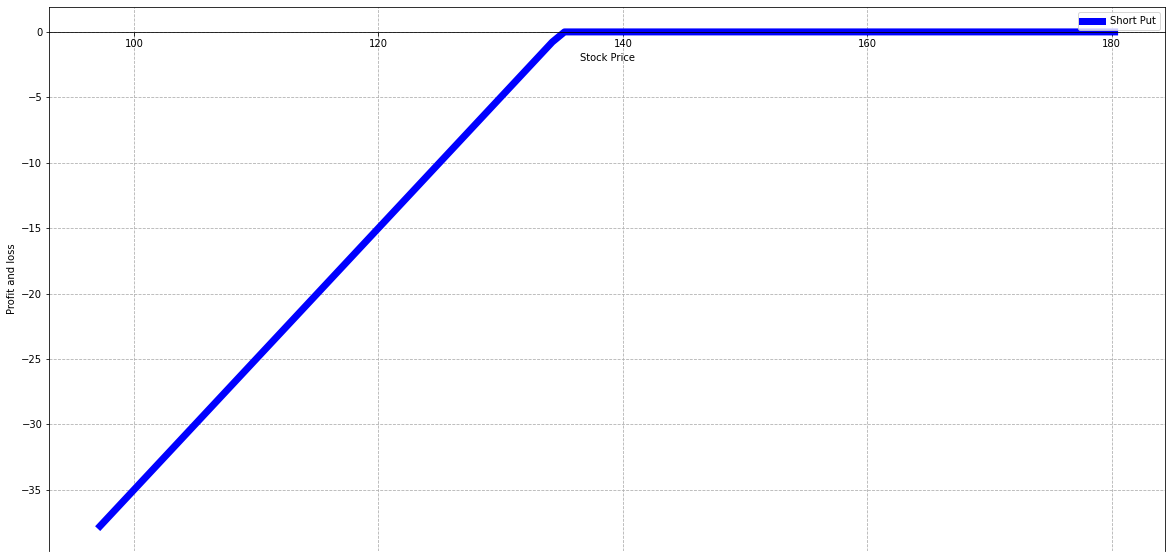
\includegraphics[width=1\textwidth]{Short_put}
		\end{center}
	\end{minipage}
	\caption{ Short Position}
\end{figure}

A put option is a contract that is agreed between the writer or seller and the holder, or buyer. The buyer has the option, but not the responsibility, to sell the underlying security at the striking price and on the termination date. The asset is regarded as the buyer. The contract is guaranteed by the seller, who, upon request, agrees to purchase the asset at the strike price on the expiration date.
This is specifically a European put. In contrast, an American put allows the holder to exercise the option at any time up until the expiration date. We will only consider European choices for the time being.
The call option and put option are presented individually in these diagrams based on their relative positions.   

\subsection{European and American Options}
A contract's price is referred to as the exercise price or strike price, and its date as the expiration date or maturity. Up until the expiration date, American options can be exercised whenever you want. Only the expiration date itself is a valid date for exercising European options. American options make up the majority of those traded on exchanges. One contract on the exchange-traded equity option market typically entails the purchase or sale of 100 shares. In general, European options are simpler to analyze than American options, and many of the characteristics of an American option can be inferred from those of its European equivalent.

\subsection{Exotic and Path Dependent Options}
A path dependent option is an exotic option whose value is influenced by the underlying asset's journey as well as its price across all or a portion of the option's life. Path-dependent options come in a variety of forms, such as Asian, Chooser, Lookback, and Barrier options.\\
The right, but not the responsibility, to buy or sell an underlying asset at a particular price, known as the strike, before or at the expiration date is provided by all options. At the beginning of the contract, options specify the strike price and expiration date. Profitability is often determined by comparing the current market price of the underlying asset to the strike price. However, the price that is utilized to calculate profitability in a path dependent option can change. Profitability may be determined, for instance, by an average price or a high or low price.


\subsection{Barrier options}
A barrier option specifies a second price in contrast to the strike price, the
barrier. Situationally, the barrier may work to activate the choice or invalidate it.
upon the kind. If the barrier price is crossed in the case of a "knock-out" barrier,
The choice loses all value. The situation with a "knock-in" barrier is the
An alternative is presented.
In all likelihood, the cost of a knockout type + the cost of a knockin type
equivalent to the cost of a standard European choice. This suggests that the cost
is always lower than that of its European counterpart for a barrier choice. Their
One benefit of a barrier option is its lower cost.

\section{Put-Call Parity}

\begin{tcolorbox}
	%[colback={red!150!brown!20},coltitle={purple}]
	[colback=Pastel Blue]
	\begin{definition}
		The value of a European call (C) with a specific exercise price (K) and exercise date (T) can be calculated from the value of a European put (P) with the same exercise price and date, and vice versa, if S represents the stock price of a non-dividend paying stock. Put-Call Parity refers to this relationship between the underlying asset and its options.
	\end{definition}
\end{tcolorbox}

$$P+S=C+k\exp[-rT+rt]$$

\noindent For European options, there is a notion known as put-call parity. As they have the same underlying asset, strike price, and expiration date, these options are considered to be of the same class. American options, which can be exercised at any time before the expiration date, are exempt from this rule.

\noindent According to put-call parity, having a short European put and a long European call of the same class at the same time will produce the same return as holding a single forward contract on the same underlying asset, with the same expiration and a forward price equal to the option's strike price.
\section{Risk-Neutral Valuation}
A probability measure called a risk neutral measure is employed in mathematical finance to help with the valuation of derivatives and other financial instruments. In order to determine the accurate price for a given asset, investors must take into account risk neutral measures, which provide a mathematical interpretation of the market's overall risk aversion.

Equilibrium measures and comparable martingale measures are other names for risk neutral measures. 
\section{Stochastic Process}
Stochastic is a technical term meaning random. A system that changes over time while being subject to random fluctuations is said to be in a stochastic process. Such a system can be explained by creating a family of random variables, $(X,t)$,where X, t represents the aspect of the system that is of interest at time t. For instance, X, t might represent the quantity of clients waiting in a line at time t. Customers will come and go as time goes on, changing the value of X, t. Any value in a subset of 0, 1, 2,..., and t at any time take one of those values. $(-\infty,\infty)$, from the endless past to the endless future.
\section{\ito Lemma}
The cost of a stock option depends on the time and price of the underlying stock. In a broader sense, we might state that the price of any derivative depends on both time and the stochastic variables that underlie the derivative. Therefore, a serious student of derivatives must develop some knowledge of how stochastic function behave. Ito's lemma is a significant finding in this field that was made by mathematician K. Ito in. Assume that a variable's value x follows the Ito procedure.
\[dx=a(x,t)dt+b(x,t)dz\]
where a and b are functions of x and t and dz is a weiner process. Drift and variation rates for the variable x are a and?2, respectively. A function G of x and t follows the process, according to Ito's lemma.
\[dG=(\frac{\delta G}{\delta x}a+\frac{\delta G}{\delta t}+\frac{1}{2}\frac{\delta^2 G}{\delta x^2}b^2)dt+\frac{\delta G}{\delta x}bdz\]
where the dz is the same Wiener process. Thus, G also follows an
Ito process, with a drift rate of
\[(\frac{\delta G}{\delta x}a+\frac{\delta G}{\delta t}+\frac{1}{2}\frac{\delta^2 G}{\delta x^2}b^2)\]
and a variance rate of
\[(\frac{\delta G}{\delta x})^2b\]
It is outside the purview of this work to provide an exhaustive proof of Ito's lemma. In the chapter's appendix, we demonstrate how the lemma can be seen as an extension of well-known differential calculus results. \\
We had suggested earlier that
\[dS=\mu S dt+\sigma S dZ\]
with $\mu$ and $\sigma$ constant, is a reasonable model of stock price movements. From Ito's
lemma, it follows that the process followed by a function G of S and t is
\[dG=(\frac{\delta G}{\delta S}\mu S+\frac{\delta G}{\delta t}+\frac{1}{2}\frac{\delta^2 G}{\delta S^2}\sigma^2 S^2)dt+\frac{\delta G}{\delta S}\sigma S dz\]
Be aware that the same underlying source of uncertainty, dz, has an impact on both S and G.
This demonstrates the significance of this in the Black-Scholes-Merton findings derivation.
\section{The Black-Scholes Model}
\subsection{ Introduction}
\noindent A key idea in contemporary finance theory is the Black-Scholes model, commonly referred to as the Black-Scholes-Merton (bf BSM) model. This mathematical formula calculates the potential value of derivatives based on other financial instruments while taking other risk variables and the impact of time into account. It was created in 1973 and is currently regarded as one of the best methods for determining the price of an options contract.
\subsection{ Assumptions}
\noindent The Black-Scholes model makes certain assumptions:\\
\begin{itemize}
	\item The stock price follows the process equation \ref{eq:gmb} with $\mu$ and $\sigma$ constant.
	\item The short selling of securities with full use of proceeds is permitted.
	\item There are no transaction costs or taxes. All securities are perfectly divisible.
	\item There are no dividends during the life of the derivative.
	\item There are no riskless arbitrage opportunities.
	\item Security trading is continuous.
	\item The risk-free rate of interest r, is constant and the same for all maturities.
	\item The option is \emph{European} and can only be exercised at expiration.
\end{itemize}
Although the original Black-Scholes model did not take into account the impacts of dividends paid throughout the option's life, the model is routinely modified to account for dividends by calculating the value of the underlying stock as of the ex-dividend date. Many option-selling market makers also alter the model to take into consideration the impact of options that can be exercised prior to expiration.
\subsection{ Methodology}
\noindent We assume that the stock price process is
\begin{equation}
	dS=\mu S d t+\sigma SdW 
	\label{eq:gmb}
\end{equation}
where $\sigma$ is the volatility, $\mu$ is risk free interest rate and $dW$ is winner process.\\[2mm]
Suppose that $C(S;t)$ be the value of an European option. To derive the {\bf BSM} model, we construct a portfolio of one long option position and a short position in some
quantity $\Delta$ of the underlying:
$$
\Pi=C(S, t)+\Delta S
$$
Over the time interval $d t$ the gain in the value of the portfolio is $t$ is
$$
d \Pi=d C(S, t)+\Delta d S
$$
i.e.
$$
d \Pi=\left(\frac{\partial C}{\partial t} d t+\mu S \frac{\partial C}{\partial S}+\frac{1}{2} \sigma^{2} S^{2} \frac{\partial^{2} C}{\partial S^{2}}\right) d t+\sigma S \frac{\partial C}{\partial S} d W+\Delta(\mu S d t+\sigma S d W)
$$
We now observe that if $\Delta=-\frac{\partial C}{\partial S}$ then the stochastic terms cancel so that the gain is deterministic.
$$
d \Pi=\left(\frac{\partial C}{\partial t} d t+\mu S \frac{\partial C}{\partial S}+\frac{1}{2} \sigma^{2} S^{2} \frac{\partial^{2} C}{\partial S^{2}}\right) d t+\sigma S \frac{\partial C}{\partial S} d W-\frac{\partial C}{\partial S}(\mu S d t+\sigma S d W)
$$
i.e.
$$
d \Pi=\left(\frac{\partial C}{\partial t} d t+\frac{1}{2} \sigma^{2} S^{2} \frac{\partial^{2} C}{\partial S^{2}}\right) d t
$$
Since there is no random term, the portfolio is riskless. By the no-arbitrage principle, a riskless portfolio must earn a risk free return . So, we have
$$
\begin{aligned}
	\frac{d \Pi}{\Pi} &=r d t \\
	\Rightarrow d \Pi &=\Pi r d t \\
	\Rightarrow d \Pi &=\left(C-\frac{\partial C}{\partial S} S\right) r d t
\end{aligned}
$$
Equating these two expressions for $d \Pi$ we find that
$$
\frac{\partial C}{\partial t} d t+\frac{1}{2} \sigma^{2} S^{2} \frac{\partial^{2} C}{\partial S^{2}}=\left(C-\frac{\partial C}{\partial S} S\right) r
$$
Hence,\\
	\begin{equation}
		\frac{\partial C}{\partial t}+\frac{1}{2} \sigma^{2} S^{2} \frac{\partial^{2} C}{\partial S^{2}}+r S \frac{\partial C}{\partial S}-r C=0
		\label{eq:bsm}
	\end{equation}

\noindent This is the \emph{Black-Scholes equation} for the value of an option.\\[2mm]
The most famous solutions to the differential equation are the Black–Scholes–Merton formulas for the prices of European call and put options. These formulas are:\\
	$$
	C=S_0N(d_1)- Ke^{-rT} N(d_2)
	$$
	$$
	P= Ke^{-rT} N(-d_2)- S_0N(-d_1)
	$$

Here
$$
\begin{aligned}
	d_{1} &=\frac{\ln \left(S_{0} / K\right)+\left(r+\sigma^{2} / 2\right) T}{\sigma \sqrt{T}} \\
	d_{2} &=\frac{\ln \left(S_{0} / K\right)+\left(r-\sigma^{2} / 2\right) T}{\sigma \sqrt{T}}=d_{1}-\sigma \sqrt{T}
\end{aligned}
$$
where the function $N(x)$ is the cumulative probability distribution function for a variable with a standard normal distribution.
\subsection{ Pricing European Options}
\noindent The Black–Scholes–Merton formula  for the prices of European call is
\begin{equation}
	C=S_0N(d_1)- Ke^{-rT} N(d_2)
	\label{eq:callprice}
\end{equation}
Where
$$
\begin{aligned}
	d_{1} &=\frac{\ln \left(S_{0} / K\right)+\left(r+\sigma^{2} / 2\right) T}{\sigma \sqrt{T}} \\
	d_{2} &=\frac{\ln \left(S_{0} / K\right)+\left(r-\sigma^{2} / 2\right) T}{\sigma \sqrt{T}}=d_{1}-\sigma \sqrt{T}\\
	N(x)&=\frac{1}{\sqrt{2 \pi}} \int_{-\infty}^{x} e^{-\frac{1}{2} y^{2}} d y
\end{aligned}
$$
Formula for the prices of European put is
\begin{equation}
	P=Ke^{-r(T-t)} N(-d_2)-S_0N(-d_1) 
	\label{eq:putprice}
\end{equation}

\subsection{ Pricing American Options}
\noindent Unlike European counterparts, American options can be exercised at any date prior to expiration. This seemingly innocent variation makes the analysis of American options much more complex. Since at each time we have to determine not only the option value but also for each value of S. At each time t, there is a particular value of S which marks the boundary between two regions: one side one should hold the option and to the other side one should exercise it. This is called a free boundary problem. There may be several such values, for instance we suppose that there is just one denoting this value varies with time by $S_f(t)$ and refer to it as the optimal exercise price.
An American call option for non-dividend-paying stock whose price is governed by a geometric Brownian motion process and stock price given by
$$
S({\mathrm{t}})=S_{0} \exp \left(\sigma W(t)+\left(r-\frac{\sigma^{2}}{2}\right) t\right)
$$
with $r$ denoting as usual the riskless rate of interest, and $\sigma$ denoting the constant volatility, $r$ and $\sigma$ are constants. 

	% !TEX root = holder_flie.tex

\chapter{Monte Carlo Method and Option Pricing}
%%

\section{Introduction}
\noindent The Monte Carlo Simulation, which uses a large number of random numbers, may prove to be a better alternative when there is a high level of uncertainty for estimating or predicting, as opposed to just replacing the uncertain variable with a single average number.\\[2mm]
For processes that are difficult to forecast because of the involvement of random variables, Monte Carlo methods are used to model the likelihood of various outcomes. It is a method for comprehending how risk and uncertainty affect forecasting and prediction models.
\section{Monte Carlo Simulation History}
Since chance and random results are essential to the modeling technique, just as they are to games like roulette, dice, and slot machines, Monte Carlo simulations are called after the well-known gambling location in Monaco.
Stanislaw Ulam, a mathematician who worked on the Manhattan Project, invented the method initially. Ulam kept himself occupied after the war while he recovered from brain surgery by playing endless rounds of solitaire. He developed an interest in graphing the results of each of these games so that he could examine their distribution and calculate the likelihood of winning. John Von Neumann and he worked together to create the Monte Carlo simulation after sharing their concept.
\section{History of Monte Carlo in Finance}
David B. Hertz published an essay in the Harvard Business Review in 1964 outlining the use of Monte Carlo methods in corporate finance, which was the first to bring them to the attention of the finance industry. Phelim Boyle was the first to employ simulation in the valuation of derivatives in his key Journal of Financial Economics work from 1977.\\[2mm]

%%\ref{https://www.youtube.com/channel/UCUcpVoi5KkJmnE3bvEhHR0Q}


\section{A Practical Example with Code}
\noindent Dart problem is a nice illustration for best comprehending the Monte Carlo approach. In this issue, we'll assume that there is a square with side 2 units, and that there is a circle with radius 1 units inside the square. Now that we know the probability of striking the circle if we toss a dart into the square, we must throw the dart at random.\\[2mm]

Therefore, on a 2-D plane with a domain defined as a square with a side of 2 units and centered on (0,0). Imagine a circle with the same radius as the square—one unit—within the same domain. The ratio between the number of points inside the circle and the overall number of points generated is then determined. \\
the area of that circle is $C=\pi$ \\
the area of that square is $S=4$ \\
the ratio would be
$\frac{C}{S}=\frac{\pi}{4}=\frac{\text{no. of points in }C}{\text{no. of points in }S}$\\[2mm]

we have to generate some random numbers for (x, y) then test it if it satisfies the following inequality 
$$x^2+y^2<=1$$. 


However, the frequency interpretation of probability informs us that as the number of trials rises, the approximation becomes more precise. Let's increase the number of trials and plot the results to see why this is the case. I ran simulations between 100 and 1000 times. Below is a display of the simulations' outcomes.\\

\subsection{Convergence of Monte Carlo}
\begin{figure}[H]
	\begin{center}
		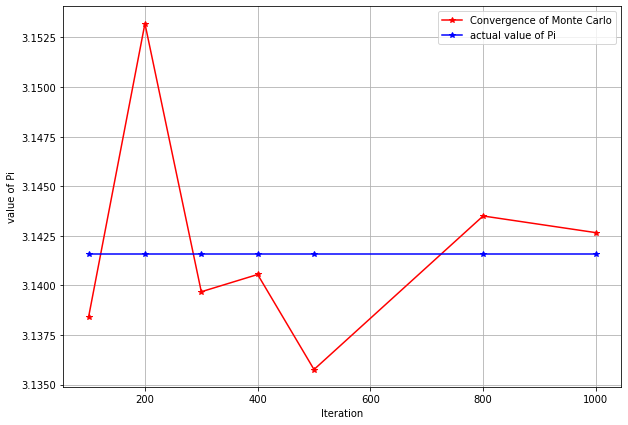
\includegraphics[width=0.8\textwidth]{dart_prob}
	\end{center}
	\caption{Convergence of Monte Carlo}
\end{figure}

\noindent From this graph we can say that MC method can converge to its actual value if we increase the number of iteration. 


\begin{table}[H]
	\begin{center}
		\begin{NiceTabular}{|c|c|c|}[hvlines]
			\rowcolor{cyan!20} Serial No. & Interval & Output  \\ 
			1 & 100 & 3.1384 \\
			2 & 200 & 3.1532 \\
			3 & 300 & 3.13968 \\
			4 & 400 & 3.14055 \\
			5 & 500 & 3.13576  \\ 
			6 & 800 & 3.1435  \\ 
			7 & 1000 & 3.14266  \\
			
		\end{NiceTabular}
	\end{center}
	\caption{Monte Carlo Method for Dart Problem}
\end{table}
%\url{https://colab.research.google.com/drive/1VQ95AiamlMWGvvWfpMmaV1nH_NNBiNgG?usp=sharing}


\section{Option Pricing}
\noindent We assess analytical solutions known as "vanilla options" for the most fundamental scenarios, such as European puts and calls. These equations are the first and most often used because they are simple to employ, sometimes even in situations when they are not quite appropriate. Contrarily, Monte Carlo is always appropriate, even though in some circumstances the solution calls for considerable dexterity. One of these occurs when future knowledge is required to make judgments in the present. It holds true for American choices. We'll look at how simulation can help tackle the problem of advanced knowledge.

The bulk of non-vanilla possibilities, however, are only path-dependent, do not call for expert knowledge, and are easily managed. We must first think about the standard scenario before we investigate unconventional solutions. It is simple to value the option at the ending price ST, discount the value back to time 0, and value the option if the option's price is not path dependent. The option's price is determined by averaging these values across a sufficient number of samples because this is only one sample.

\subsection{Monte Carlo as a tool for Financial Math}
\noindent We'll learn more about the Monte Carlo simulation technique for pricing financial derivatives right now. Only by employing the financial mathematics of risk-neutral pricing and modeling risk-neutral asset pathways is the valuation of financial derivatives through Monte Carlo simulations conceivable.\\
\begin{equation}
	\frac{C_{t}}{B_{t}}= E_{Q}[\frac{C_{T}}{B_{T}}|F_{t}]
\end{equation}
\subsection{Computationally inefficient}
\noindent In its most fundamental form, Monte Carlo is inefficient when compared to the straightforward mathematical equations that are available for some deterministic PDEs, such as the Black-Scholes option pricing model for European Options. The method for pricing sophisticated derivatives is, of course, the main factor in our decision to choose Monte Carlo.

In any case, we can improve the accuracy by using:
\begin{itemize}
	\item Antithetic Variates.\\[-4mm]
	\item Control Variates
\end{itemize}
\subsection{Valuation by Simulation}
\noindent According to the method of risk-neutral pricing, an option's value equals the risk-neutral expectation of its discounted payment.
By calculating the mean of many deferred payoffs, we can estimate this expectation. Regarding a certain simulation, i:

\begin{equation}
	C_{0,i}= C_{T,i}e^{\int_{0}^{T}-r_{s}\,ds}\\
\end{equation}
\begin{equation}
	C_{0,i}=e^{-rT}C_{T,i}
\end{equation}

\noindent Now if we repeat the simulation M times, we can average the outcomes.\\
\begin{equation}
	\hat{C}_{0}=\frac{1}{M} \sum_{i=1}^{M} C_{0,i}
\end{equation}
\noindent \^{C} is an estimate of the true value of the option 
C\textsubscript{0} with error due to the fact we are taking an average of randomly generated samples, and so therefore the calculation is itself random. A measure of this error is the standard deviation of 
\^{C} called the standard error. This can be estimated as the standard deviation of C\textsubscript{0,i} divided by the number of samples M.
$$SE(\hat{C}_{0})=\frac{\sigma(C_{0,i})}{\sqrt{M}}$$ 

%$${\sigma(C_{0,i})}=\sqrt{\frac{1}{M-1}\[ \sum_{i=1}^{M} (C_{0,i}-\hat{C_{0}})^2\]}}$$
\subsection{European Call Option in the Black-Scholes World}
\noindent Here we have constant interest rate so the discount factor is exp(-rT) and the stock dynamics are modelled with Geometric Brownian Motion GBM.
$$dS_{t}=rS_{t}dt+\sigma S_{t}dW_{t}$$
Let’s simulate this GBM process by simulating variables of the natural logarithm process of the stock price
$$x_{t}=ln(S_{t})$$ 
which is normally distributed. For the dynamics of the natural logarithm process of stock prices under GBM model we need to use Ito’s calculus.
$$dx_{t}=vdt+\sigma dz_{t}$$
$$v=r-\frac{1}{2}\sigma^2$$
We can then discretize the Stochastic Differential Equation SDE by changing the infinitesimals dx,dt,dz into small steps $\Delta x$,$\Delta t$,$\Delta z$
$$\Delta x=v\Delta t+\sigma\Delta z$$
This is the exact solution to the SDE and involves no approximation.
$$x_{t+\Delta t}=x_{t}+v\Delta t+\sigma(z_{t+\Delta t}-z_{t})$$
In terms of the stock price S, we have:
$$S_{t+\Delta t}=S_{t}\exp({v\Delta t+\sigma(z_{t+\Delta t}-z_{t})})$$
Where
$$(z_{t+\Delta t}-z_{t}) \sim N(0,\Delta t)\sim \sqrt{\Delta t}N(0,1) \sim \sqrt{\Delta t}\epsilon_{i}$$

\subsection{Algorithm} 
\noindent Monte Carlo continuous pricing algorithm\\
inputs:  \\
$S, K, vol, r, N, M, T$ \newline
Steps:
$dt=T/N$ \newline
$nudt=(r-0.5vol^2)*dt$  \newline
$volsdt=volsqrt(dt)$  \newline
$sumCT=0$  \newline
$sumCT2=0$  \newline
\indent $lnSt=lnSt+nudt+volsdt*epsilon$  \newline
\indent $ST=exp(lnSt)$  \newline
\indent $CT=max(0,ST-k)$  \newline
\indent $sumCT=sumCT+CT$  \newline
\indent $sumCT=sumCT2+CT*CT$  \newline
$C0=exp(-rT)sumCT/M$  \newline


\subsection{Result}

\begin{table}[H]
	\begin{center}
		\begin{NiceTabular}{|c|c|c|c|}[hvlines]
			\rowcolor{cyan!20} Maturity & Strike Price & Option Price & Standard Error\\ 
			\Block{7-1}{1} & \Block{7-1}{100} & 3.83 & 0.11 \\ 
			& & 3.65 & 0.11 \\
			& & 3.73 & 0.12 \\
			& & 3.53 & 0.1  \\
			& & 3.77 & 0.11 \\
			& & 3.88 & 0.11 \\
			& & 3.84 & 0.11 \\
		\end{NiceTabular}
	\end{center}
	\caption{Monte Carlo Method for European Call}
\end{table}


\noindent Applying monte carlo method we can see a slide deviation from its actual value. Moreover, the standard error is on average 0.11.

\subsection{Option Price with Maturity}



\begin{table}[H]
	\begin{center}
		\begin{NiceTabular}{|c|c|}[hvlines]
			\rowcolor{cyan!20} Maturity & Option Price\\ 
			0.01 & 3.11 \\ 
			0.02 & 3.09 \\
			0.03 & 3.17 \\
			0.04 & 3.15  \\
			0.05 & 3.17 \\
			0.06 & 3.29 \\
			0.07 & 3.33 \\
		\end{NiceTabular}
	\end{center}
	\caption{Monte Carlo Method for European Call Maturity}
\end{table}

\noindent Keeping the strike price same we have made this table of maturity and option price. Here, we can see a linear relationship between these two factors. 
\begin{figure}[H]
	\begin{center}
		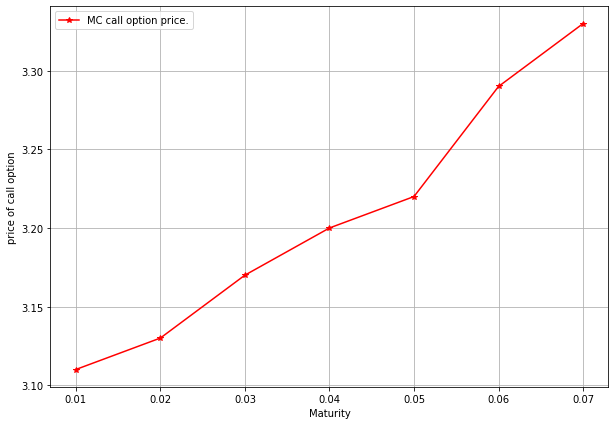
\includegraphics[width=0.8\textwidth]{MC_call_option_price}
	\end{center}
	\caption{Option Price with Maturity}
\end{figure}



\subsection{Relation Between Option Price and Strike Price}



\begin{table}[H]
\begin{center}
	\begin{NiceTabular}{|c|c|}[hvlines]
		\rowcolor{cyan!20} Strike Price & Option Price\\ 
		60 & 41.22 \\ 
		70 & 31.14 \\
		80 & 21.25 \\
		90 & 11.23  \\
		100 & 1.76 \\
	\end{NiceTabular}
\end{center}
	\caption{Option Price and Strike Price}
\end{table}


\begin{figure}[H]
	\begin{center}
		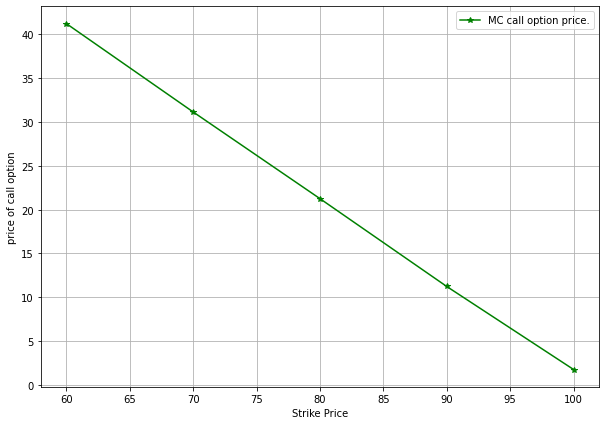
\includegraphics[width=0.8\textwidth]{MC_Strike_Price}
	\end{center}
	\caption{Relation Between Option Price and Strike Price}
\end{figure}
\section{Monte Carlo Variance Reduction Methods – Antithetic}
\noindent We will now come up with a concept for lowering the variance of the Monte Carlo simulation method while valuing financial derivatives. Unfortunately, while being a fantastic strategy for estimating option values with complex payoffs or high dimensionality, we must run a lot of simulations M in order to obtain an acceptable level of accuracy. Instead, we can rely on strategies for variance reduction, which follow the same rules as hedging an option position. i.e., a hedged option portfolio's volatility will be lower than that of its unhedged equivalent.
\subsection{Antithetic Variates}
\noindent Let’s write an option on asset $S_{1}$
and another option on asset $S_{1}$
that is perfectly negatively correlated with $S_{1}$ and which currently has the same price. $S_{1}$
and $S_{2}$ satisfy the following Stochastic Differential Equations:
$$dS_{1,t}=rdS_{1,t}dt+\sigma dS_{1,t}dz_{t}$$
$$dS_{2,t}=rdS_{2,t}dt+\sigma dS_{2,t}dz_{t}$$
The value of these two options is equal because the two assets' prices and volatilities are the same. The volatility of the pay-off of a portfolio that includes both of these contracts, however, is substantially lower than the variance of the pay-off of each contract separately. We are essentially reducing the significant peak in the probability distribution associated with a single contract pay-off. Basic Intuition, i.e., the idea that when one choice succeeds, the other does not.
\subsection{Implementation of Antithetic Variate}
\noindent We generate a fictitious asset that is perfectly negatively linked with the real asset in order to apply an antithetic variate. The process of implementation is quite straightforward, and if we use the European Call Option as an example, our simulated pay-offs fall under the following categories: 
$$S_{t+\Delta t}=S_{t}\exp(v\Delta t+\sigma(z_{t+\Delta t}-z_{t}))$$
Where
$$(z_{t+\Delta t}-z_{t}) \sim N(0,\Delta t)\sim \sqrt{\Delta t}N(0,1) \sim \sqrt{\Delta t}\epsilon_{i}$$

\noindent Contract Simulation
$$-C_{T,i}=max(0,S \exp(v\Delta T+\sigma\sqrt{T}(\epsilon_{i}))-K)$$
$$-\bar{C}_{T,i}=max(0,S \exp(v\Delta T+\sigma\sqrt{T}(-\epsilon_{i}))-K)$$
\subsection{Algorithm} 
\noindent Monte Carlo continuous pricing algorithm\\
inputs:  \\
$S, K, vol, r, N, M, T$ \newline
Steps:
$dt=T/N$ \newline
$\nu dt=(r-0.5vol^2)*dt$  \newline
$volsdt=volsqrt(dt)$  \newline
$sumCT=0$  \newline
$sumCT2=0$  \newline
\indent $lnSt=lnSt+nudt+volsdt*epsilon$  \newline
\indent $ST=exp(lnSt)$  \newline
\indent $CT=max(0,ST-k)$  \newline
\indent $sumCT=sumCT+CT$  \newline
\indent $sumCT=sumCT2+CT*CT$  \newline
$C0=exp(-rT)sumCT/M$  \newline
\sub{\subsection{Result}}

\begin{center}
\begin{NiceTabular}{|c|c|c|}[hvlines]
	\rowcolor{cyan!20} Option Price & SE & Computation Time\\ 
	7.47 & 0.324 & 0.4867\\ 
	7.97 & 0.331 & 0.4845\\
	7.63 & 0.334 & 0.4916\\
\end{NiceTabular}
\end{center}


\subsection{Option Price with Strike Price}

\begin{center}
	\begin{NiceTabular}{|c|c|}[hvlines]
		\rowcolor{cyan!20} Strike Price & Option Price\\ 
		60 & 41.2 \\ 
		70 & 31.21 \\
		80 & 21.23 \\
		90 & 11.23  \\
		100 & 1.73 \\
	\end{NiceTabular}
\end{center}

\begin{figure}[H]
	\begin{center}
		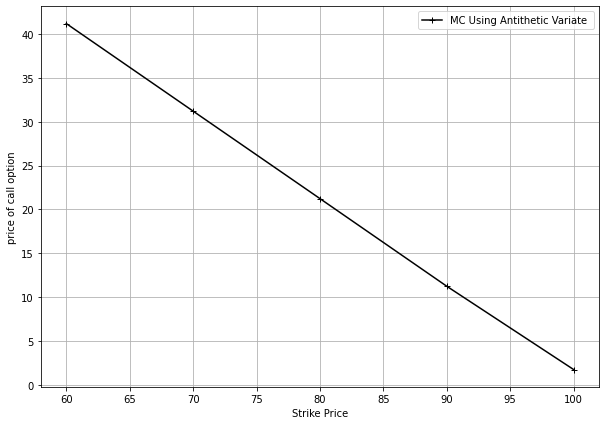
\includegraphics[width=0.8\textwidth]{mc_antithetic}
	\end{center}
	\caption{Option Price with Strike Price}
\end{figure}

\section{Pricing an Up-and-Out Barrier Option}
\sub{\subsection{Path-Dependent option}}
\noindent The barrier option is a well-liked product when pricing complex or exotic path dependant options. These options have a conventional European option expiration style, but they only become active if the underlying price reaches a predetermined barrier threshold. This barrier level may be monitored continuously or intermittently. $\tau$
For an up-and-out barrier put option:
$$C_{T}=f(S_{T})=(K-S_{T})^+ind( max S_{t}<H)$$

\sub{\subsection{Algorithm}}
\noindent Monte Carlo continuous pricing algorithm\\
inputs:  \\
$S0, K, H, vol, r, N, M, T$ \newline
Steps:
$dt=T/N$ \newline
$\nu dt=(r-0.5vol^2)*dt$  \newline
$volsdt=volsqrt(dt)$  \newline
$sumCT=0$  \newline
$sumCT2=0$  \newline
For $i:$  \newline
\indent $BARIER= FALSE$ \newline
\indent $St=S0$ \newline
\indent For $j:$ \newline
\indent\indent $lnSt=lnSt+nudt+volsdt*epsilon$  \newline
\indent\indent $ST=exp(lnSt)$  \newline
\indent\indent $CT=max(0,ST-k)$  \newline
\indent\indent $sumCT=sumCT+CT$  \newline
\indent\indent $sumCT=sumCT2+CT*CT$  \newline
\indent\indent if BARRIER: \newline
\indent\indent\indent CT=0 \newline
\indent\indent else: \newline
\indent\indent\indent $CT=max(0,K-St)$ \newline
$C0=exp(-rT)sumCT/M$  \newline
\sub{\subsection{Result}}


\begin{center}
\begin{NiceTabular}{|c|c|c|}[hvlines]
	\rowcolor{cyan!20} Option Price & SE & Computation Time\\ 
	7.47 & 0.324 & 0.4867\\ 
	7.97 & 0.331 & 0.4845\\
	7.63 & 0.334 & 0.4916\\
\end{NiceTabular}
\end{center}

\sub{\subsection{Option Price with Maturity}}

\begin{center}
	\begin{NiceTabular}{|c|c|}[hvlines]
		\rowcolor{cyan!20} Maturity & Option Price\\ 
		0.01 & 0.7 \\ 
		0.02 & 1.09 \\
		0.03 & 1.55 \\
		0.04 & 1.56  \\
		0.05 & 1.76 \\
		0.06 & 2 \\
		0.07 & 1.91 \\
	\end{NiceTabular}
\end{center}

\begin{figure}[H]
	\begin{center}
		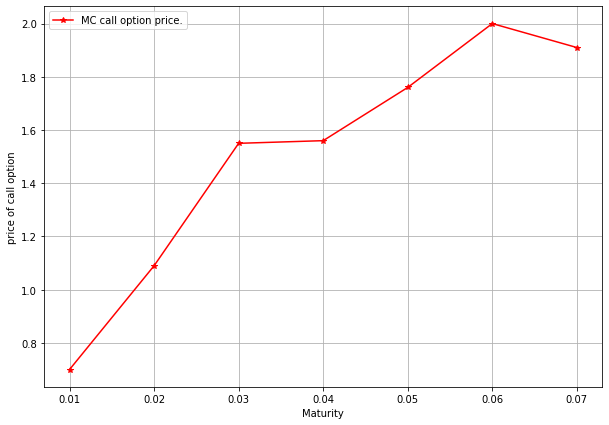
\includegraphics[width=0.8\textwidth]{MC_Barrier_Option_With_Maturity}
	\end{center}
	\caption{Option Price with Maturity}
\end{figure}

\sub{\subsection{Relation Between Option Price and Strike Price}}

\begin{center}
	\begin{NiceTabular}{|c|c|}[hvlines]
		\rowcolor{cyan!20} Strike Price & Option Price\\ 
		100 & 1.88 \\ 
		110 & 10.15 \\
		120 & 19.87 \\
		130 & 30.01  \\
		140 & 40.06 \\
	\end{NiceTabular}
\end{center}

\begin{figure}[H]
	\begin{center}
		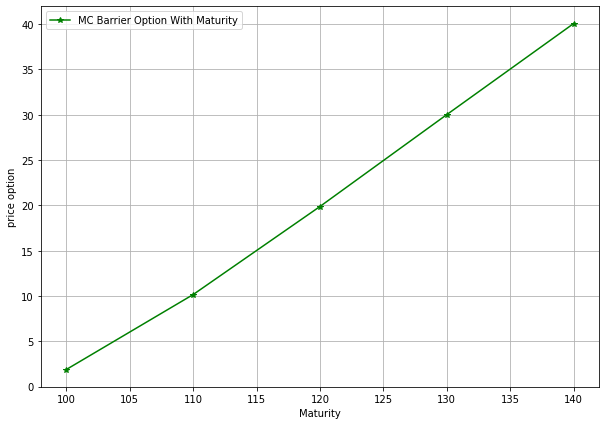
\includegraphics[width=0.8\textwidth]{MC_Barrier_Option_With_Strike_Price}
	\end{center}
	\caption{Option Price and Strike Price}
\end{figure}


\sub{\subsection{The Monte Carlo Method for American Options}}
\noindent As we've seen, the fundamental binomial approach can calculate American option pricing with just a simple and minor change. This is due to the fact that the backward technique works by first determining option prices at expiration and then working backwards to the beginning date. As a result, every time an early exercise is an option, it is simple to decide not to exercise because it is known what the option's future value will be if it is not. Furthermore, there are only two potential outcomes for the future value in question.
A forward technique, however, lacks this kind of future knowledge. Think about the challenge a GRW will face when the option is well-positioned to win at some point in the walk. Even if the discounted expiration value of the option were known at that point, for instance by applying the Black-Scholes formula, the knowledge would not be adequate because there might be additional opportunities for early exercise before expiration. As a result, the option's discounted expiration value does not appropriately reflect its value at the time in question.
However, there is a zone in which, depending on the amount of time left before expiration, the option should be exercised early if it were sufficiently deep in the money. The idea of an exercise boundary is derived from this one.

\sub{\subsection{Algorithm}} 
\noindent Monte Carlo continuous pricing algorithm\\
inputs:  \\
$S_0,T,k, r,\Delta t, \sigma, N$ and the exercise boundary B(t) \newline
$E=0$\\
$n=T/\Delta t$\\
for $i=1,...N$  \newline
\indent $S=S_{0}$\\
\indent for $t=\Delta t,2\Delta t,...n\Delta t$\\
\indent $Z \sim N(0,1)$  \newline
\indent $S_{t}=S_{t-1}(1+rt+\sigma\sqrt{\Delta t}Z)$\\ %\newline
\indent \indent if $K-S_{t}>=KB(T-t)$\\
\indent \indent \indent $E=E+\exp(-rT)(k-S_{t})$ \\ 
\indent \indent \indent go to next i\\
\indent\indent endif\\
\indent end for t
\indent $E=E+\exp(-rT)(k-S_{t})$ \\ 
end for i\\
$E=\frac{E}{N}$ \newline
option price=$\exp(-rT)E$  \newline


\begin{center}
	\begin{NiceTabular}{|c|c|c|c|c|}[hvlines]
		\rowcolor{cyan!20} T & K & European Option & American Option & SE \\ 
		\Block{9-1}{1}& 80 &   0.6812 &   0.6886 &   0.0108 \\
		& 85 &   1.3607 &   1.3657 &   0.0037 \\ 
		& 90 &   2.3019 &   2.4913 &   0.0823 \\
		& 95 &   3.7361 &   3.9601 &   0.0600 \\
		& 100 &   5.6507 &   6.0940 &   0.0784 \\
		& 105 &   7.8782 &   8.7486 &   0.1105 \\
		& 110 &  10.6292 &  11.9784 &   0.1269 \\
		& 115 &  13.6376 &  15.7496 &   0.1549 \\
		& 120 &  17.2459 &  20.1122 &   0.1662 \\
	\end{NiceTabular}
\end{center}

\begin{figure}[H]
	\begin{center}
		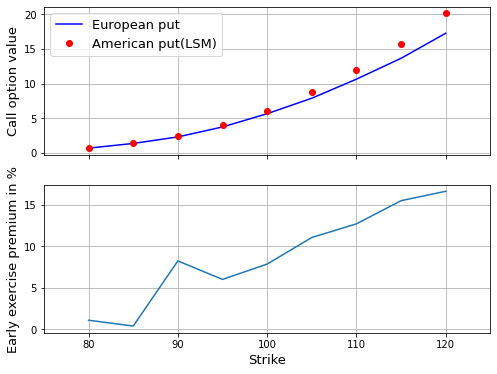
\includegraphics[width=0.8\textwidth]{American_option}
	\end{center}
	\caption{American Put Option}
\end{figure}
	% !TEX root = holder_file.tex
\chapter{Comparison}
\section{Black Scholes vs All}
\subsection{European Call option: Black Scholes Method vs Monte Carlo Method}

Here, We will create a table for European Call option pricing by Monte Carlo method(with 1000
simulations) using computer generated pseudorandom numbers and then compare those
values with Black-Scholes method results. We are taking stock price, S = 30, strike price, K = From 40 to 60, volatility, vol = 0.3, risk-free rate, r = 0.01, T=1

\begin{table}[H]
\begin{center}
	\begin{NiceTabular}{|c|c|c|c|c|}[hvlines]
		\rowcolor{cyan!20} T & K & BSM & MC & Abs. Diff \\ 
		\Block{5-1}{1}& 40 &   0.98 &   0.78 &   0.2 \\
		& 45 &   0.48 &   0.36 &   0.12 \\
		& 50 &   0.23 &   0.26 &   0.03 \\ 
		& 55 &   0.11 &   0.16 &   0.05 \\
		& 60 &   0.05 &   0.04 &   0.01 \\
	\end{NiceTabular}
\end{center}
\caption{BSM vs MC for European Call}
\end{table}

\noindent Table 4.1 shows that for five different iteration, the difference of BSM and MC is very small. So, MC Method can be told as a good approximation method for evaluating option price.

\subsection{European Call option: Black Scholes Method vs Antithetic}

Here, We will create a table for European Call option pricing by Monte Carlo method(with 1000
simulations) using computer generated pseudorandom numbers and then compare those
values with Black-Scholes method results. We are taking stock price, S = 30, strike price, K = From 40 to 60, volatility, vol = 0.3, risk-free rate, r = 0.01, T=1


\begin{table} [H]
\begin{center}
	\begin{NiceTabular}{|c|c|c|c|c|}[hvlines]
		\rowcolor{cyan!20} T & K & BSM & Antithetic & Abs. Diff \\ 
		\Block{5-1}{1}& 40 &   0.98 &   0.9 &   0.08 \\
		& 45 &   0.48 &   0.41 &   0.07 \\
		& 50 &   0.23 &   0.25 &   0.02 \\ 
		& 55 &   0.11 &   0.11 &   0.0 \\
		& 60 &   0.05 &   0.03 &   0.02 \\
	\end{NiceTabular}
\end{center}
\caption{BSM vs Antithetic}
\end{table}

\noindent Table 4.2 reflects that for five different iteration, the difference of BSM and Antithetic is lower then the previous one. Antithetic is a variance reduction method. So, it increases the efficiency of MC Method and reduces the computation time.

\begin{figure}[H]
	\begin{center}
		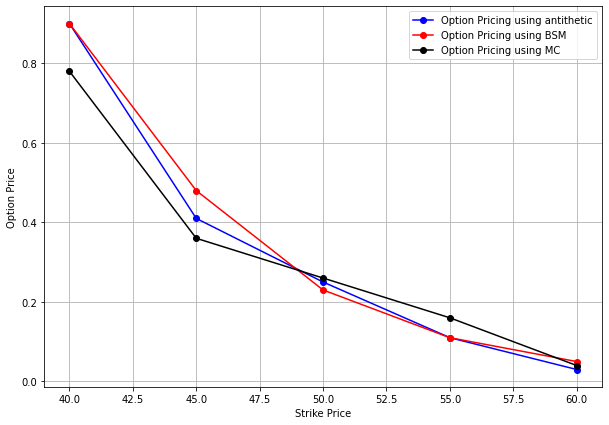
\includegraphics[width=0.8\textwidth]{Option_Pricing_Using_Different_Method}
	\end{center}
	\caption{Option Pricing Using Different Method}
\end{figure}


\noindent Figure 4.1 portrays the movement of option price with respect to strike price for BSM, MC and Antithetic. If we consider BSM as the standard, we can see that the MC and Antithetic is showing good results. In fact, Antithetic is giving better approximation. 

\begin{figure}[H]
	\begin{center}
		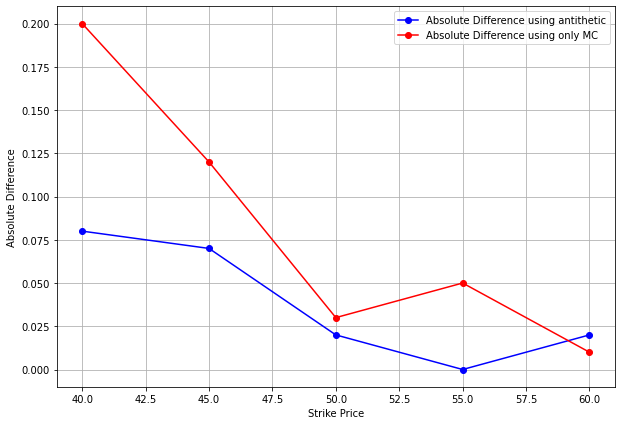
\includegraphics[width=0.8\textwidth]{Absolute_Difference_for_MC_and_Antithetic}
	\end{center}
	\caption{Absolute Difference for MC and Antithetic}
\end{figure}

\noindent From figure 4.2, the absolute difference for Antithetic is lower then MC method.  

\subsection{Barrier Put option: Black Scholes Method vs Monte Carlo Method}

Here, We will create a table for European Call option pricing by Monte Carlo method(with 1000
simulations) using computer generated pseudorandom numbers and then compare those
values with Black-Scholes method results. We are taking stock price, S = 30, strike price, K = From 40 to 60, volatility, vol = 0.3, risk-free rate, r = 0.01, T=1


\begin{table} [H]
\begin{center}
	\begin{NiceTabular}{|c|c|c|c|c|}[hvlines]
		\rowcolor{cyan!20} T & K & BSM & MC & Abs. Diff \\ 
		\Block{5-1}{1}& 40 &   10.59 &   10.77 &   0.18 \\
		& 45 &   15.03 &   15.19 &   0.16 \\
		& 50 &   19.73 &   19.99 &   0.26 \\ 
		& 55 &   24.56 &   24.8 &   0.24 \\
		& 60 &   29.45 &   29.16 &   0.29 \\
	\end{NiceTabular}
\end{center}
\caption{BSM vs MC for Barrier Put}
\end{table}


\noindent Table 4.3 shows that for five different iteration, the difference of BSM and MC is very small. So, MC Method can be told as a good approximation method for evaluating option price of Barrier Put Option.

\begin{figure}[H]
	\begin{center}
		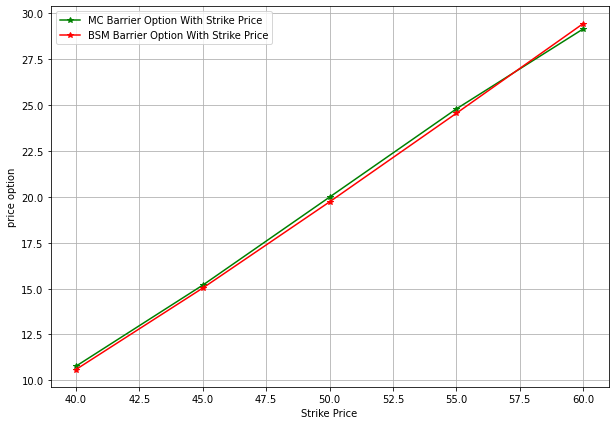
\includegraphics[width=0.8\textwidth]{barrier_mc_bsm}
	\end{center}
	\caption{For Barrier Option MC and BSM With Strike Price}
\end{figure}

\begin{figure}[H]
	\begin{center}
		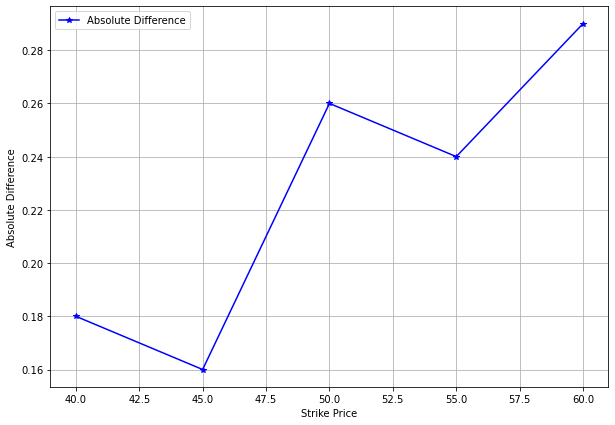
\includegraphics[width=0.8\textwidth]{For_Barrier_Option_Absolute_Difference}
	\end{center}
	\caption{For Barrier Option Absolute Difference}
\end{figure}


\noindent Figure 4.4 shows the absolute difference. As these iterations has been run by some random numbers, values are fluctuating. 
	% !TEX root = holder_file.tex
\chapter{Conclusion}
	\noindent In this project, we have discussed various topics related to derivatives, in particular options, namely, European, American and Barrier. We have used Monte Carlo Simulation Method for pricing these options. \\[2mm]
	
	\noindent We have shown MC method for European Call option. In table 4.1 we can see that the absolute difference is very low of BSM and MC. So, Monte Carlo Method is an excellent method for evaluating option prices. But this method is computationally inefficient. If we increase the number of iteration, it would take a long time to compute the result. So, for reducing the computational cost and saving time, we have discussed some variance reduction method specially Antithetic Method. After using this, the approximation become better. 
	\noindent Moreover, we have shown same output for American Call Option and Barrier Put Option. In both cases, Monte Carlo Method is showing results which are almost matching to BSM Method. 
	\noindent Here, we’ve implemented these procedures discussed in this
	project into Python coding for numerical results as well as graphical representation. We also have a fantastic experience throughout our project
	using the most scientific typesetting  \LaTeX . Finally, we like to conclude that this
	work will be a good guideline for further study of pricing other options like exotic
	options, asian options etc.
	\appendix
	% !TEX root = holder_flie.tex

\chapter{Some Codes}
%%
%%https://towardsdatascience.com/monte-carlo-simulations-with-python-part-1-f5627b7d60b0
\sub{\subsection{Code for Dart Problem}}
\lstinputlisting[language=Python]{a_practical_example_with_code.py}
\sub{\subsection{Code for Monte Carlo}}
\lstinputlisting[language=Python]{monte_carlo.py}
\sub{\subsection{Code for Antithetic}}
\lstinputlisting[language=Python]{antithetic.py}
\sub{\subsection{Code for Barrier Option}}
\lstinputlisting[language=Python]{pricing_an_up_and_out_barrier_option.py}
	
	\begin{thebibliography}{99}
		\bibitem{hull} {J. C. Hull.}, Options, futures, and other derivatives. $8^{\text{th}}$ ed. Upper Saddle River, NJ: Prentice Hall, 2012. 
		\bibitem{wilmott} {P. Wilmott, S. Howison, and J. Dewynne.} The mathematics of financial derivatives. A student introduction. Cambridge: Cambridge Univ. Press., 1995.
		\bibitem{Shonkwiler} {R. W. Shonkwiler} Finance with
		Monte Carlo. Springer, 2013.
		\bibitem{clewlow} {L. Clewlow, C. Strickland} Implementing Derivatives Models. John Wiley and Ltd, 2007.
		\bibitem{Brandimarte} {P. Brandimarte} Numerical Models in Finance and Economics $2^{\text{nd}}$. JOHN WILEY AND SONS, INC., 2006.
		\bibitem{JACQUIER} {A. JACQUIER, E. R. MALONE, AND M. OUMGARI} Stacked Monte Carlo for option pricing. JOHN WILEY AND SONS, INC., 2019.
		\bibitem{Goodman} {J. Goodman} Lecture Notes on Monte Carlo Methods. Courant Institute of Mathematical Sciences, NYU, 2005.
	\end{thebibliography}
	
\end{document}
